\documentclass[10pt,twocolumn,letterpaper]{article}

\usepackage{cvpr}
\usepackage{times}
\usepackage{epsfig}
\usepackage{graphicx}
\usepackage{amsmath}
\usepackage{amssymb}

\graphicspath{{pictures/}}
% Include other packages here, before hyperref.

% If you comment hyperref and then uncomment it, you should delete
% egpaper.aux before re-running latex.  (Or just hit 'q' on the first latex
% run, let it finish, and you should be clear).
\usepackage[breaklinks=true,bookmarks=false]{hyperref}

\cvprfinalcopy % *** Uncomment this line for the final submission

\def\cvprPaperID{****} % *** Enter the CVPR Paper ID here
\def\httilde{\mbox{\tt\raisebox{-.5ex}{\symbol{126}}}}

% Pages are numbered in submission mode, and unnumbered in camera-ready
%\ifcvprfinal\pagestyle{empty}\fi
%\setcounter{page}{4321}
\begin{document}

%%%%%%%%% TITLE
\title{Optimal Lobotomy}

\author{Clement Lee\\
Princeton University\\
{\tt\small clem@princeton.edu}\\
\emph{advised by Jianxiong Xiao}
}
\maketitle
%\thispagestyle{empty}

%%%%%%%%% ABSTRACT
\begin{abstract}
  We highlight common works in the field of neural network optimization, and present our own findings on weight deletion methodologies.
  We experiment with Optimal Brain Damage and weight thresholding, and achieve a 20-fold reduction on the parameter space of VGG-16 with no loss in performance.
  
\end{abstract}

%%%%%%%%% BODY TEXT
\section{Introduction}

Deep learning techniques abound in the modern literature, with a primary focus on achieving higher and higher levels of accuracy.
In general, models have been getting increasingly larger to accommodate improvements in techniques, and computational costs of machine learning have been rising accordingly.
Pointedly, the rate of development of deep learning models has far outstripped actual hardware improvements.
Specialized techniques are being continually introduced to handle bigger models, such as in Dean et al \cite{dean2012large}, who construct a distributed deep learning system.
However, due to fundamental restrictions in the basic architecture, the optimal node count for their system is relatively low, and scaling is a continual problem that requires careful tuning of parameters.

Distributing neural networks tends to be difficult, as they are fundamentally based on large matrix multiplications which do not lend themselves to partitioning.
Thus, most parallelization approaches tend to focus on \emph{data parallelization}, which splits up the training data into smaller chunks and runs the model on each chunk, accumulating gradient parameters at the end of each minibatch.
This, however, does not solve the problem of large models, for which it is impossible to perform data parallelization.
The only way forward is with \emph{model parallelization}, which splits the model into smaller chunks that can be processed on each node, and then combines the results.
This comes with its own difficulties to solve, such as the speed of this synchronization step, but provides a potential and reasonable architecture for parallel training and execution.

It is of further primary interest to train models on a GPU cluster rather than a traditional CPU setup, as multiple orders of magnitude of performance improvements  are commonly possible when training typical convolutional neural networks.
However, GPUs are commonly far more limited in memory than an average server, and a high-end NVIDIA GTX Titan X has only 12GB of memory.
Due to the necessary parameters necessary for gradient-based algorithms, this can easily be filled when training midsized models.
Thus, efficient usage of this memory is a key problem, and remains largely untackled by common algorithms.

Neural networks are also generally extremely over-dimensioned for their tasks.
Many training algorithms are designed around increasing the relative ``importance'' of each weight connection, and methods like dropout follow a similar goal.
In the case of dropout, this is entirely based by the high-level assumption that many of the parameters can entirely be switched-off (many standard dropout implementations assume 50\% as a default).
Considering specific models, AlexNet, a common baseline convolutional network, contains 61 million trainable parameters, and VGG-16, a more modern network, contains 138 million trainable parameters.
It is an increasing trend in the literature to reconsider the necessity of these parameters, as they result in longer training times and much more complicated computational demands.

In this paper, we explore the possibility of reducing the parameter space of networks automatically, without the necessity for costly amounts of human intervention.
The primary aim is to produce a smaller but performant network through the application of prior weight-reduction algorithms, which have generally been focused on extremely small networks.
We utilize various weight deletion policies to highlight the possibility of greatly reducing network sizes with minimal or insignificant impact on performance.

\subsection{Related Work}
\paragraph{Distributed Machine Learning}
Lee et al \cite{lee2014model} build a system for distributing a network across multiple nodes in a potentially high-latency cluster.
Their work is interesting for its application of gradient aggregation, canonized by a specific set of instructions.
They produce near-linear scaling on CPU cluster training, which is an interesting result in light of general cluster inefficiencies (speed of synchronization, suboptimal work division, etc.).
This suggests that deep learning training is often bottlenecked not by actual processing speed but by other factors, such as memory bandwidth.
Indeed, there is evidence that even NVIDIA's highly optimized cuDNN codepath cannot saturate GPU usage during typical training loads, and loading data onto a GPU for training is a significant hurdle.

\paragraph{Hybrid Data/Model Parallelization}
Methodologies that combine data and model parallelization have also been proposed by Krizhevsky \cite{krizhevsky2014one}.
This attempts to tackle the problem using domain-specific optimizations, and does not affect the actual model itself. 
It also does not cover the case where the model is itself too large for memory, and thus is limited in its direct application to this work, though its demonstrated scaling (around 6-fold for a 8-node cluster) is impressive and indicates that parallelization can potentially yield immense benefits for both training and execution speed.
These results are corroborated by Yadan et al \cite{yadan2013multi}, who demonstrate good speedups by utilizing both kinds of parallelism.

\paragraph{Binary Networks}
Networks that simplify floating-point operations done on GPUs down to simple binary operations that can be efficiently performed on a CPU have been proposed by Rastegari et al \cite{rastegari2016xnor}.
They trim AlexNet down using binary operations with only a 2.9\% loss in accuracy, resulting in 32-fold memory savings.
This supports the general hypothesis that neural networks generally contain far more data than is necessary to operate, and thus weights can be largely reduced without significant impact on the network.
This maintains the same number of parameters, but merely affects the information encoded in each one.

\paragraph{Efficient filters}
There is significant evidence in the literature indicating that smaller floating-point networks can achieve similar results to benchmarks while being considerably more efficient: SqueezeNet, by Iandola et al \cite{iandola2016squeezenet} achieves a 50-fold reduction in parameter space at no cost to performance.
This required a carefully designed architecture, as well as specifically tuned hyperparameters.
This indicates that common models for deep learning have memory capacity that largely surpasses their learning capacity---that is, even with currently leading learning algorithms, models are not efficiently using their parameters for optimal performance.

\subsection{Limitations}
We believe that in the general literature, automatic weight reduction schemes are not commonly considered, as primary focus tends to be on models that have been carefully designed for their specific task.
We aim to build an algorithm that is independent of human intervention, and requires a minimum of tuning.
Towards this goal, we synthesize the key findings from the related work, namely the implicit network inefficiencies, and attempt to use these to guide our experiments.

One of the key difficulties of model parallelization is distributing the computation evenly and efficiently among multiple computing nodes.
This requires both a reduction in linked computation (that requires expensive synchronization), and an actual splitting of the work.
With that aim in mind, we focus in this paper on reducing the parameter space and not explicitly on the split process, which we leave to further investigation.

\section{Weight Deletion}
We explore the 
\subsection{Optimal Brain Damage}
In terms of early results in weight removal, LeCun et al \cite{lecun1989optimal} construct the optimal brain damage algorithm, which utilizes the diagonal elements of the parameter's Hessian matrix (second derivatives) to calculate an approximation of the effect of each weight.
They hypothesize that the non-diagonal elements are likely to be 0, and generally unimportant.
This work defines the \emph{saliency} of a weight: that is, the importance of weight relative to the other weights in the network.
Intuitively, this is guided by the fact that weights are trained on the first derivative of the error, so the second derivative should be the impact of each weight on the total error.

This, however, is dependent on the loss function being used, and can thus be a rather involved calculation for more complicated tasks.
The cross-entropy loss, a commonly used loss function for classification tasks, has a far more complex second derivative and is thus difficult to calculate well.
As such, we limit our experiments with OBD to smaller size networks, and test it for large scale parameter reduction.
We also explore optimizations and approximations to the base algorithm, by estimating the second derivative without doing the full calculation.

\subsection{Optimal Brain Surgeon}
Hassibi et al \cite{hassibi1993optimal, hassibi1994optimal} propose an improvement on the optimal brain damage algorithm, noting that the assumption of diagonality on the Hessian matrix is likely to be flawed.
They instead calculate the full matrix, and use this to select the optimal weight to delete.
They note that for extremely small networks trained on the XOR problem, their weight removal algorithm is the only one to delete weights without compromising the entire network's learning capacity.
That is, other algorithms irreversibly delete weights prevent the network from learning the problem at all.

This enhanced calculation is promising, but unfortunately runs into an extremely fatal problem when tackling modern networks: by calculating the full Hessian matrix, it requires $O(n^2)$ space to hold the second derivatives of each pair of weights.
This is entirely unrealistic for modern networks, where we consider network size $n$ to be in the millions.
We, however, take note of their analyses, which note that OBD and weight magnitude pruning may be closer in performance than original calculations had suggested.
As such, we rely on the overarching ideas on the weight deletion framework to motivate our findings, but our intention is to extend it to larger networks.
\subsection{Weight Thresholding}
We propose a simpler methodology, inspired by the assumption that weights are generally plentiful and can be reduced \emph{en masse} before any significant impact is made on the network.
Simple investigation on the distribution of network weights indicated that the mean was roughly around 0, but that the standard deviation was in fact very low.
This indicated that there were large numbers of weights that had been trained to extremely low values, so we hypothesize that they can likely be removed from the network entirely.
This was explored in earlier works but the approximation does not hold as well for smaller networks.
Smaller weights can also still have 

Importantly, it is an etremely

As the 
\section{Experiments}
We run two primary experiments, one with the full OBD algorithm, and one based on our proposal algorithm.

\subsection{Small network}
As the OBD algorithm is rather computationally expensive, we try a smaller sample test on a fully-connected network.
This network is meant to approximate to sine function, so it takes in a value $x$ between 0 and $2\pi$.
We construct a network of 2 hidden layers of 20 neurons each, applying the tanh transfer function after each layer, and train for 3000 iterations on batch sizes of 10000 randomly-generated examples using the mean-squared-error loss function.
This gives us a trained MSE of 0.047, recalling that for this specific training case, a score of 0.5 is no different from random number generation.
For our experiments on this network, we incrementally delete weights one by one (from a total of 481 parameters).

For this to be run efficiently, we utilize common $\epsilon$-approximations of the gradient, which introduce small amounts of floating-point error into the calculation, but are generally considered small enough not to impact calculations significantly.
These are inspired by similar results as implemented in Torch, the software package we use to 

\paragraph{Without retraining} Our first experiment is in simply deleting weights without retraining the network at all, simply to see how the weights are used.
The results are shown in Figure~\ref{fig:sin-no}, and as predicted, the 
Notably, the 

\begin{figure}[h]
  \centering
  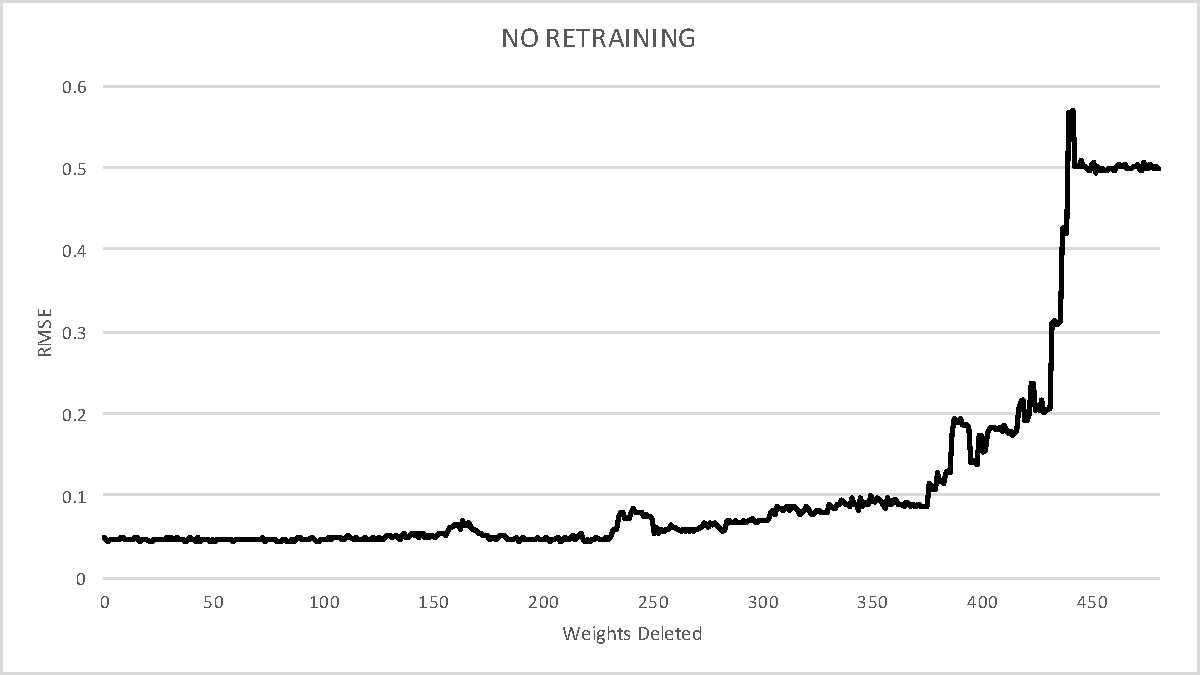
\includegraphics[width=\linewidth]{sin-no-retraining.pdf}
  \caption{Weight deletion without retraining.}
  \label{fig:sin-no}
\end{figure}


\paragraph{With retraining} As our primary goal is not to merely investigate the importance of each weight but also how they affect the overall \emph{learning capacity} of the network, we run a secondary experiment by allowing the network 100 iterations (again with batches of 10000) after each weight deletion.
This allows for significantly better results, which are shown in Figure~\ref{fig:sin-with}.


\begin{figure}[h]
  \centering
  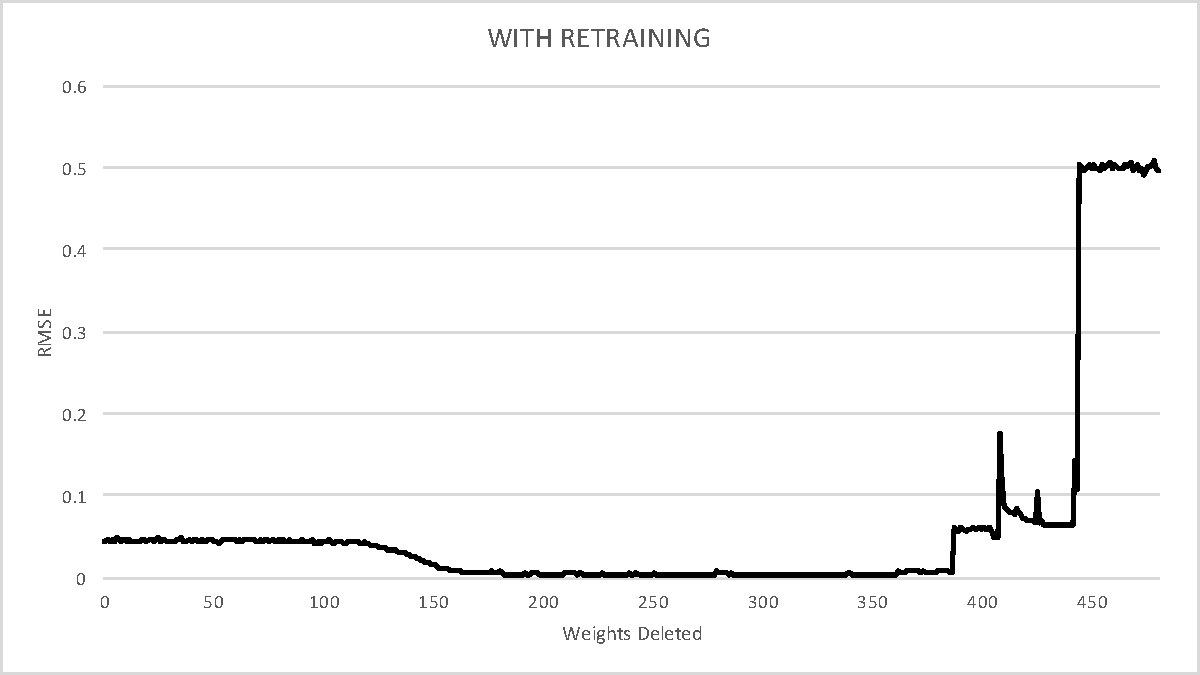
\includegraphics[width=\linewidth]{sin-with-retraining.pdf}
  \caption{Weight deletion with retraining.}
  \label{fig:sin-with}
\end{figure}

Interestingly, weight deletion followed by retraining actually allowed for better mean-squared error than the minimum that had been achieved with normal training.
The error decreases from the baseline of 0.047 down to an incredibly low 0.0015.
This points in fact to a very potentially interesting possibility that overdimensioned networks can fail to learn as well as pruned networks, and that incremental weight removal can allow for better accuracy than is possible with the original network.

This is a point of potential future exploration, as it is well-known that many networks converge onto local minima on the error.
Smaller networks are known to generally converge faster with larger perturbations on each weight, so the change of being forced into a local minima is much smaller.
Typical stochastic gradient descent methodologies are intended to avoid or ``speed past'' local minima in search of better parameters, but many techniques are in fact designed specifically to solve the problem of slow convergence (and thus poor training error) in large networks.

On the flip side, we can also see that there is a point beyond around 450 deletions where the network simply loses all ability to perform its task, and no amount of retraining (even performed after this experiment) is able to get it to regain a reasonable amount of performance.
This is particularly fascinating because it is a sudden jump from performance that was still reasonably good (around 0.07).
This suggests that there is a fundamental \emph{maximum learning capacity} of a network, which in this case is oversaturated by the problem at 30 weights.
Further investigation of this point is an interesting topic as it may reveal what kinds of network architectures are entirely necessary for different kinds of problems.

\subsection{CIFAR-10 and VGGnet}
We perform a variety of experiments on a network based on VGG-16 and trained on CIFAR-10, a common convolutional network dataset and benchmark.
Using a learning rate of 1, cut in half every 25 epochs, we run 300 epochs using the ADAM gradient descent methodology.
This results in a baseline performance of 92.22\% on our validation set.


\paragraph{Weight-based thresholding}
We note that the standard deviation of the aggregate parameters was 0.0074, and progressively threshold away weights up to 0.007.
We remove the weights in gradual steps of 0.001, and run separate trials with and without retraining, presenting our findings in Figure~\ref{fig:vgg-thresh}.
\begin{figure}[h]
  \centering
  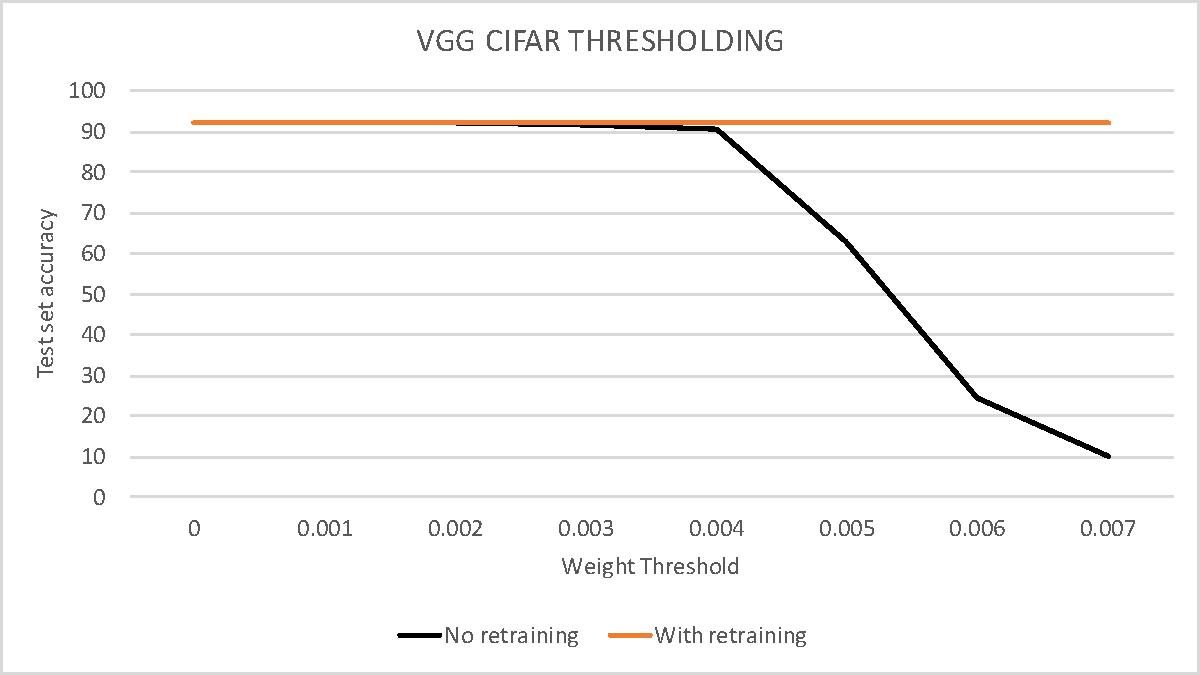
\includegraphics[width=\linewidth]{cifar-threshold.pdf}
  \caption{Weight deletion without and without retraining.}
  \label{fig:vgg-thresh}
\end{figure}

We note that we are able to delete over 87\% of the weights without having any visible impact on performance; in fact, some tests while reducing the network gave marginally better test performance than the original trained network.
This represents over 120 million deleted weights from an original network size of 138 million parameters, which indicates the viability of our methodology.

\paragraph{Top-$k$ thresholding}
Unfortunately, weight-based thresholding is largely imprecise in the number of weights deleted, making it difficult to quantize actual improvements rigorously without accidentally overstepping

\subsection{Discussion}
We analyze the distribution of weight deletion as applied by our algorithm, and show these results in Figure~\ref{fig:vgg-histo}.
We note that the early weights are very rarely deleted, which makes sense, as the early weights are the crucial convolutional layers which effectively preprocess the information.
The majority of the weights in VGG-16 are in the fully-connected layers, and we note that this is also where the rate of deletion is the highest.
The maximum of this histogram is indicated in a plateau in the middle of the graph, which represents the first fully-connected layer.
This suggests that common architectures may have far larger fully-connected layers than are necessary for their performance, and that deeper layers may have more impact.

\begin{figure}[h]
  \centering
  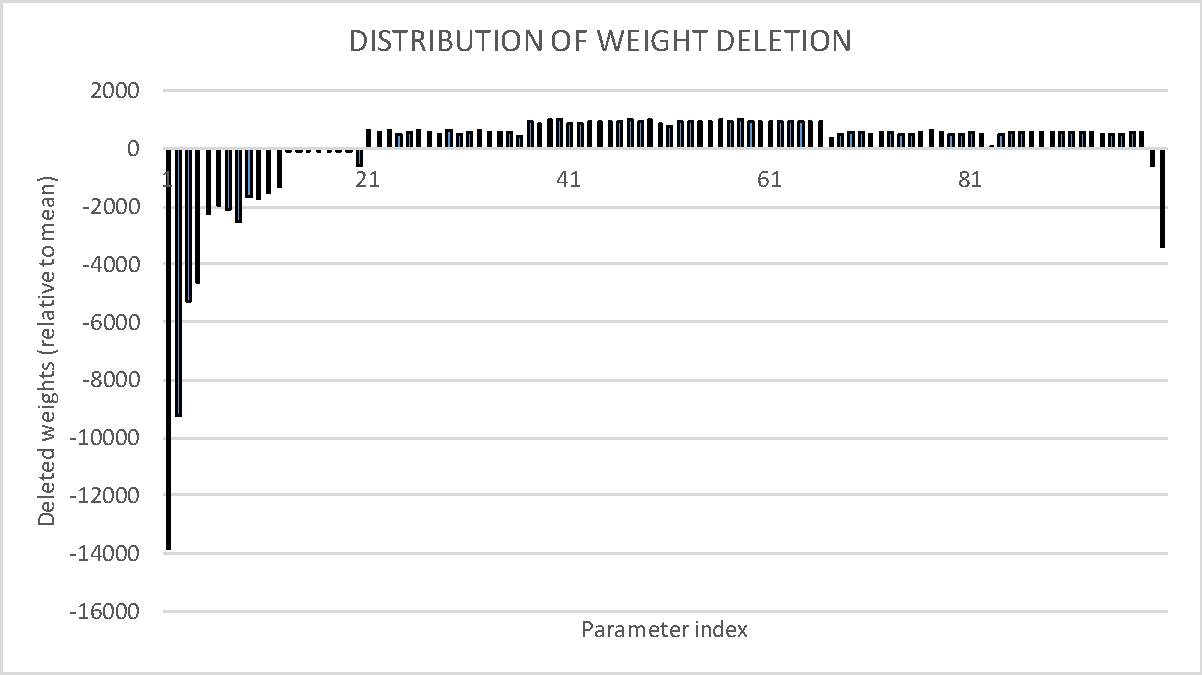
\includegraphics[width=\linewidth]{cifar-histogram.pdf}
  \caption{Histogram of where weights are deleted, relative to mean deletion rate.}
  \label{fig:vgg-histo}
\end{figure}

It is also important to note that in a convolutional layer, all of the weights are shared between every image patch the convolution is run on, so the weights are individually far more important.
In addition, the feature maps generated are crucial to the whole implementation of convolutional networks, so it is logical for their deletion rate to be far lower.
At the same time, however, it is interesting that almost 90\% of the weights are still being deleted from these early layers.
\section{Future Work}
We have demonstrated the potential for both weight deletion algorithms to reduce network capacity hugely without reducing accuracy.
However, because of algorithmic and computational limitations at the current moment, we are not able to apply the OBD algorithm in full to the larger networks.
We would like to experiment with a hybrid methodology that combines the speed of deleting small weights initially (the ``low-hanging fruit'') with a later pass of OBD on the reduced network, for which the computation will be easier.
We observe that weight thresholding can delete parameters incorrectly as we aim to approach 100-fold space savings, so we believe that improved algorithms like OBD can step in and continue the process.

We would also like to explore the possibility of using our reduced sparse network to create a partitioning: multiple fast approximate graph partitioning methods exist, and would be well suited to separating the layers into distinct and rarely-connected components.
This would allow us to achieve better space savings in practice, as we can then remove neurons as well as weights.
Furthermore, this would allow us to extend our work onto multiple GPUs and apply model parallelization to test our split network.

It is also important to test additional datasets; CIFAR-10 is one of the easier benchmarks, chosen for speed of training and ease of use.
However, we would also like to explore the applicability of our algorithm to CIFAR-100, ILSVRC-2012, and others, for which there is perhaps a fundamentally lower limit to the number of parameters that may be deleted from the network.

\section{Conclusion}
{\small
\bibliographystyle{ieee}
%just cite everything -- REMOVE LATER
\nocite{*}
\bibliography{ref}
}

\end{document}
